% Enhanced LaTeX CV for Yassine Oubaid
% This document is an updated and more complete curriculum vitae
% suitable for postdoctoral applications.  It incorporates research
% experience, large facility experiments, conferences and schools,
% teaching activities and key skills.  Feel free to adjust dates or
% details as your experience evolves.

\documentclass[13pt,a4paper]{article}
\usepackage[margin=1in]{geometry}
\usepackage[T1]{fontenc}
\usepackage{lmodern}
\usepackage{hyperref}
\usepackage{enumitem}
\usepackage{setspace}
\usepackage{tabularx}
\usepackage{array}
\usepackage{graphicx}

\newcommand{\cvdate}[1]{\makebox[0pt][r]{\small #1\hspace{-0.4em}}}

\newcommand{\cvbullet}{\textbullet\hspace{0.6em}}
% Additional packages and color definitions for styling
\usepackage{xcolor}

% --- Colors ---
\definecolor{sectionred}{RGB}{200,0,0}    % deep red
\definecolor{sectiongrey}{RGB}{90,90,90}  % medium grey (tweak as you like)
\definecolor{jobblue}{RGB}{0,0,180}       % dark blue for job titles
\definecolor{sectionblack}{RGB}{0,0,0} 
% --- Section title color switch (default = grey) ---
\colorlet{sectiontitlecolor}{sectionblack} % current section title color

\newcommand{\setsectitlecolor}[1]{\colorlet{sectiontitlecolor}{#1}}

% --- Title macros ---
\newcommand{\sectitle}[1]{\textcolor{sectiontitlecolor}{#1}}
\newcommand{\jobtitle}[1]{\textcolor{jobblue}{\textbf{#1}}}

% --- Convenience shortcuts ---
\newcommand{\sectitlegrey}{\setsectitlecolor{sectiongrey}}
\newcommand{\sectitlered}{\setsectitlecolor{sectionred}}
\newcommand{\sectitleblack}{\setsectitlecolor{black}}


% Format hyperlinks nicely
\hypersetup{
  colorlinks=true,
  linkcolor=black,
  urlcolor=blue,
  pdfauthor={Yassine Oubaid},
  pdftitle={Curriculum Vitae - Yassine Oubaid}
}

% Reduce vertical space between items
\setlist[itemize]{leftmargin=*, itemsep=0.2em}

\begin{document}


%------------------------------------------------------------------------------
% Header
%------------------------------------------------------------------------------
% Requires: \usepackage{graphicx} in the preamble

\begin{center}
\begin{tabularx}{\linewidth}{@{}l X@{}}
\raisebox{-0.7\height}{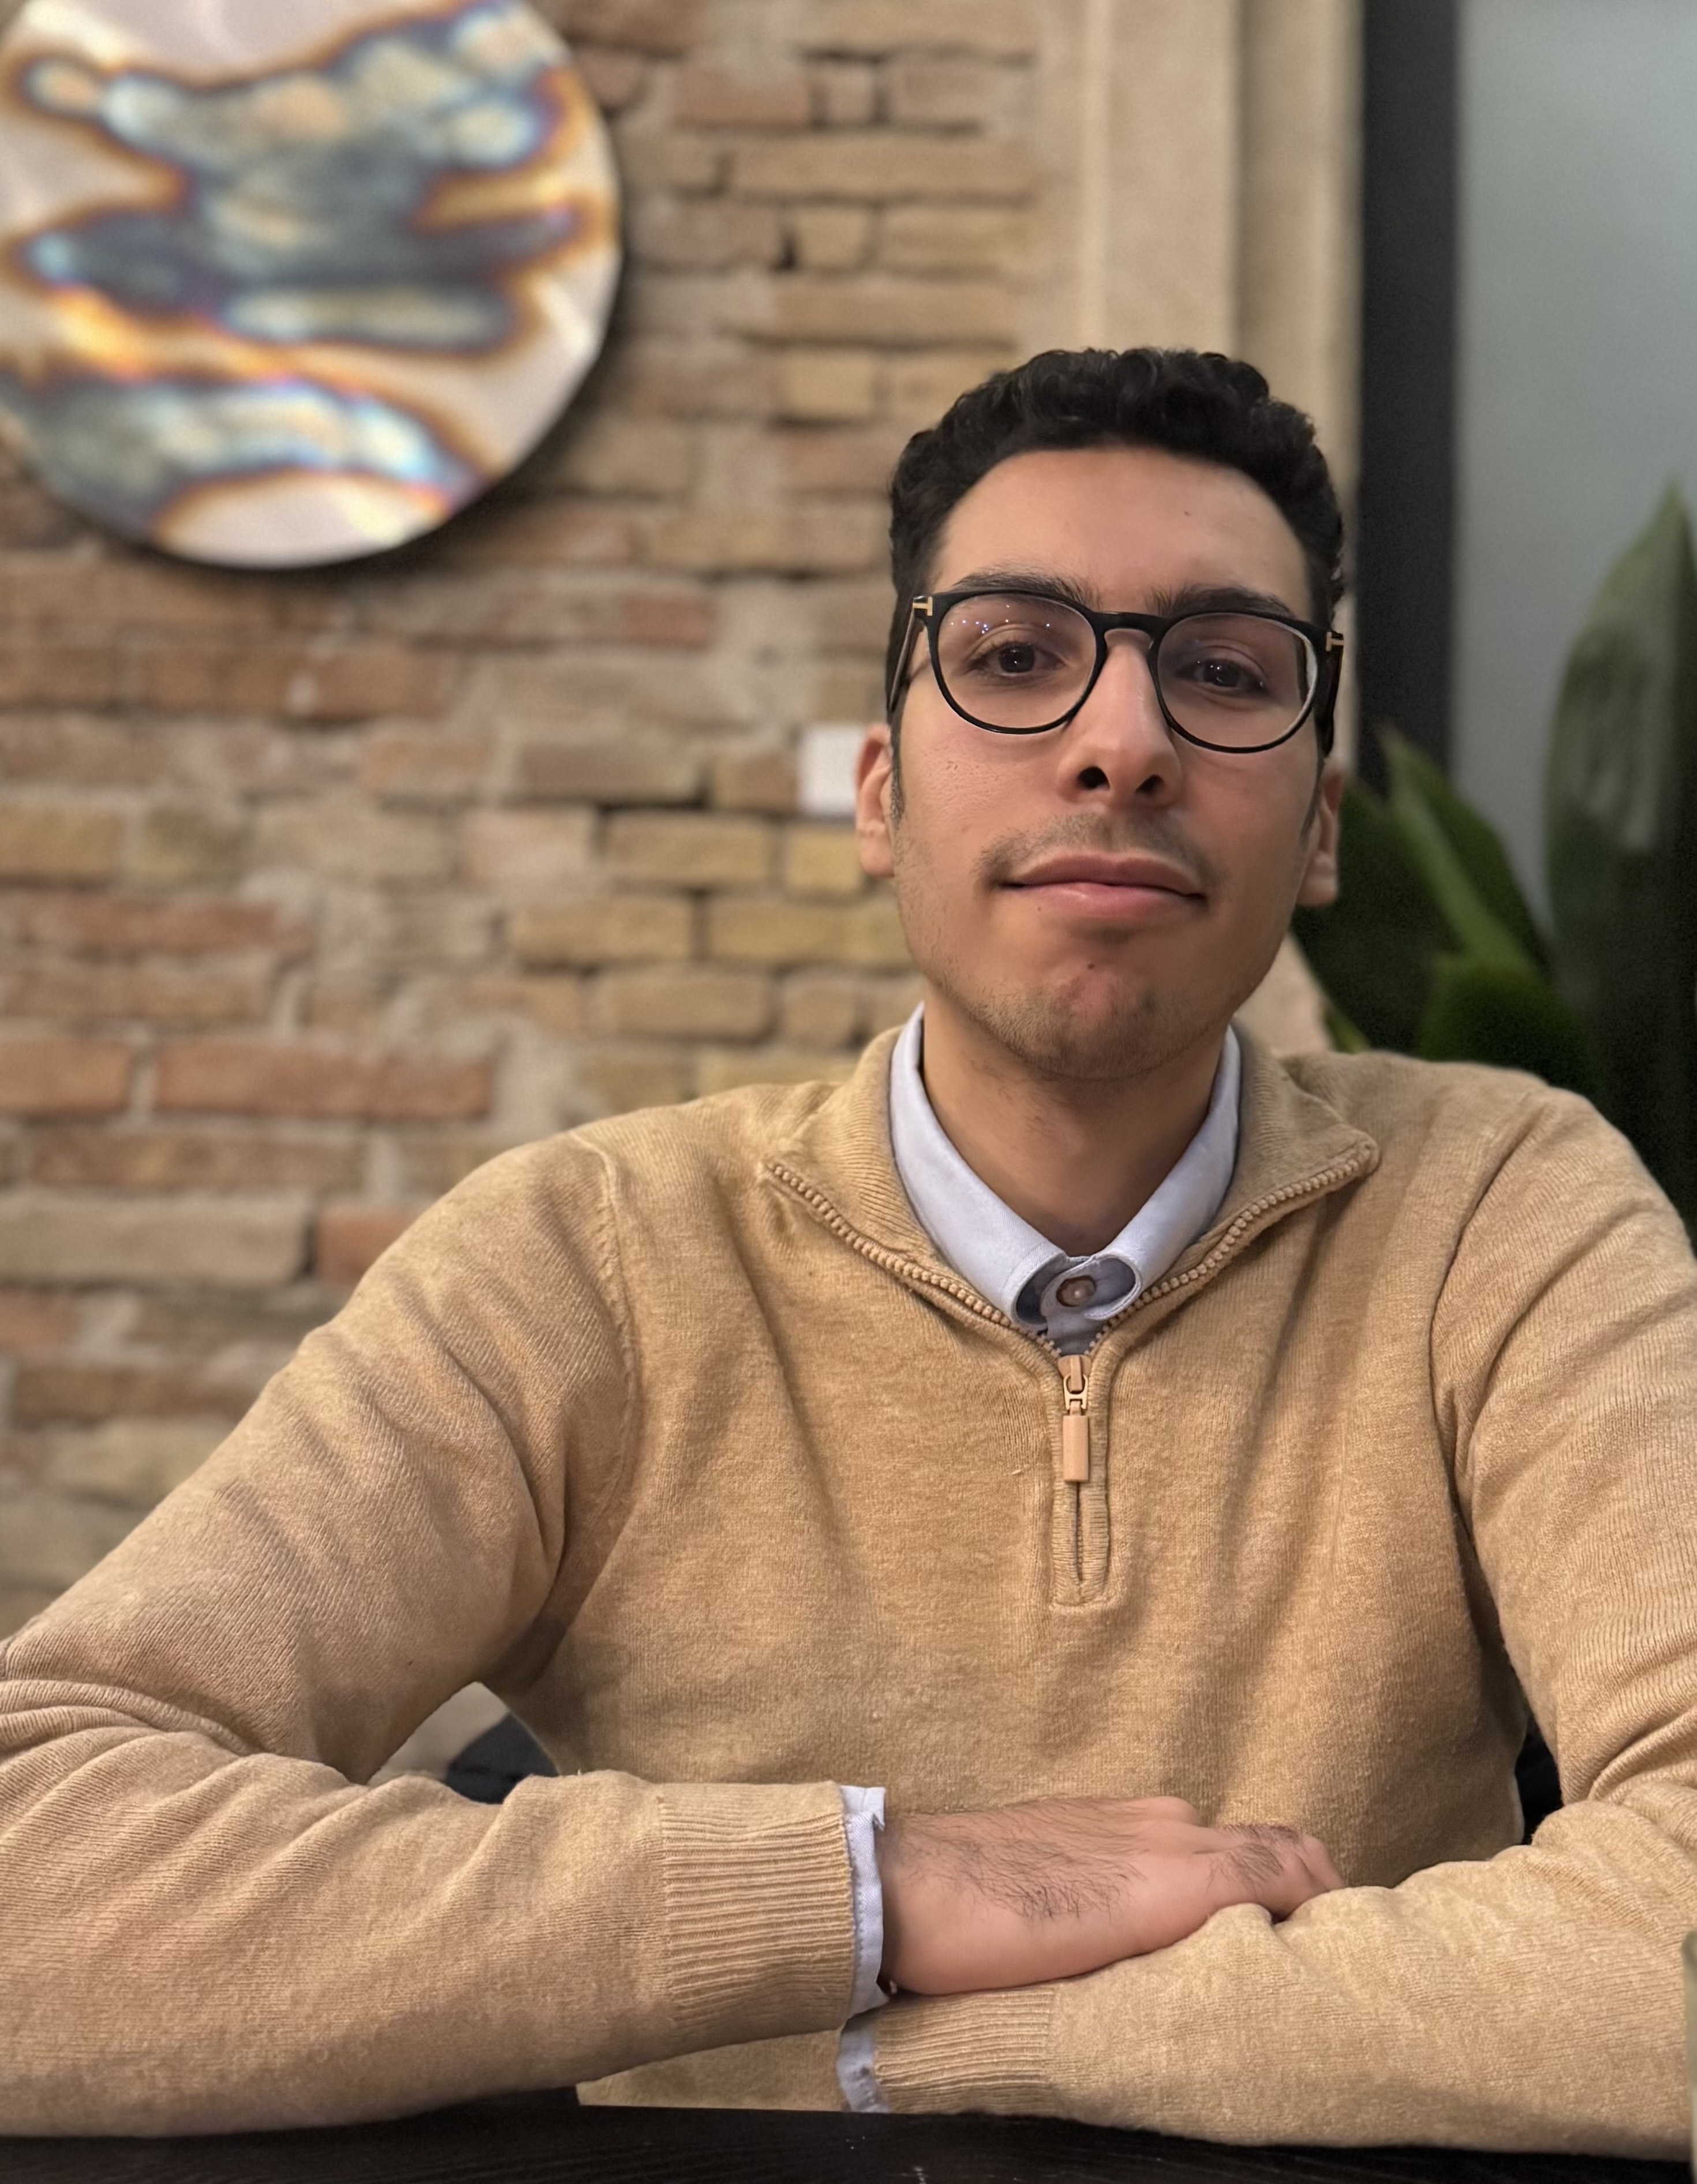
\includegraphics[width=4cm]{photo_perso.jpeg}} &
\begin{minipage}[t]{\linewidth}
{\LARGE\textbf{Yassine Oubaid}}\\[2mm]
PhD in Condensed Matter Physics\\
Université Paris--Saclay\\[2mm]
\href{mailto:yassinosoubaid@gmail.com}{yassinosoubaid@gmail.com} \quad | \quad
\href{https://scholar.google.com/citations?user=XXXXX}{Google Scholar} \quad | \quad
\href{https://orcid.org/0009-0009-9471-8382}{ORCID} \quad \\[2mm]
20 rue de Chablis, 91940 Les Ulis, France
\end{minipage}
\end{tabularx}
\end{center}


\vspace{0.5em}

%------------------------------------------------------------------------------
% Research Interests
%------------------------------------------------------------------------------
\section*{\sectitle{Research Interests}}
\begin{itemize}
  \item Strongly correlated electron systems and phase transitions
  \item Unconventional superconductors
  \item Exotic magnetism
  \item Synchrotron and neutron scattering techniques
  \item Optical spectroscopy (infrared/THz)
  \item Measurements under extreme conditions (High pressure / low temperature)
\end{itemize}

\section*{\sectitle{Education}}

\begin{tabularx}{\linewidth}{@{}p{0pt}X@{}}
\cvdate{2023--present} &
\jobtitle{PhD in Condensed Matter Physics} -- Université Paris--Saclay | SOLEIL Synchrotron \\
& | Solid state physics laboratory (LPS) \emph{(25 February 2026)}\\
& (International ranking: 6th worldwide in Physics — Shanghai Ranking 2025)\\
& Thesis: Study of the interplay of magnetism, structure, and electronic properties in the Iron-Based spin ladder BaFe$_2$S$_3$.\\
& Advisors: Pascale FOURY-LEYLEKIAN, Director of Solid state physics laboratory (LPS), Victor BAL\'EDENT, Professor, Pierre FERTEY, head of CRISTAL beamline, Marine VERSEILS, Beam scientist (AILES beamline).\\[0.9ex]
\cvdate{2021--2022} &
\jobtitle{Engineering/MSc (M2)} -- Ecole Centrale Lyon (ECL), France\\
& General engineering curriculum in Ecole Centrale Lyon with a specialisation in nanoscience and a Master in nanoscience the same year (Master Nanoscale engineering (NSE) : ECL, INSA Lyon, Université de Lyon (ULCB)).\\[0.9ex]

\cvdate{2019--2021} &
\jobtitle{Engineering Diploma} -- Ecole Centrale Casablanca, Morocco\\
& General engineering student with a nanoscience specialisation during the second year.\\
& Excellence Scholarship : Bourse fondation OCP\\[0.9ex]

\cvdate{2017--2019} &
\jobtitle{Preparatory Classes (PSI)} -- Lycée d'excellence de Benguerir (LYDEX), Morocco\\
& Ranked 30th nationwide (top 3\% of the accepted candidates)\\
\end{tabularx}

\section*{\sectitle{Research and Professional Experience}}

\begin{tabularx}{\linewidth}{@{}p{0pt}X@{}}

\cvdate{2023--present} &
\jobtitle{PhD Student -- Iron-based superconductor BaFe$_2$S$_3$}\\
& \textbf{(Université Paris--Saclay | Synchrotron SOLEIL | LPS, France)}\\
& Study of the interplay of magnetism, structure, and electronic properties in the iron-based spin ladder BaFe$_2$S$_3$.\\[0.9ex]

\cvdate{2022} &
\jobtitle{Research Internship -- Topological superconductivity in hybrid nanowires}\\
& \textbf{(CNRS (Institut Néel) | CEA (IRIG), Grenoble, France)}\\
& Tailoring superconductivity in core-shell InAs--ZnTe nanowires.\\[0.9ex]

\cvdate{2021} &
\jobtitle{Research Internship -- 2D materials growth}\\
& \textbf{(Ecole Centrale Casablanca | UM6P Benguerir, Morocco)}\\
& Contribution to a review paper on 2D materials, focusing on CVD (chemical vapor deposition) growth for FET (field-effect transistor) applications.\\

\end{tabularx}



%------------------------------------------------------------------------------
% Experimental Experience at Large Facilities
%------------------------------------------------------------------------------
\section*{\sectitle{Experiments at Large Facilities}}
\begin{itemize}
  \item \textbf{AILES beamline, Synchrotron SOLEIL (Paris):} infrared spectroscopy in : THz, Far-infrared, Mid-infrared, Near-infrared. (low temperature/high pressure).
  
  \item \textbf{CRISTAL beamline, Synchrotron SOLEIL (Paris):} Single crystal/powder X-ray diffraction. (low temperature/high pressure).

  \item \textbf{thALES, IN8 instruments, Institut Laue–Langevin (ILL) (Grenoble):} Inelastic neutron scattering.
  \item \textbf{D1B,D20 instruments, Institut Laue–Langevin (ILL) (Grenoble):} powder neutron diffraction under high pressure and low temperature.
  
  \item \textbf{D9,D23 instruments, Institut Laue–Langevin (Grenoble):} single-crystal neutron diffraction at low temperature and high magnetic field.
  
   \item \textbf{ESRF/ILL/ALBA Synchrotron:} Training experiments during HERCULES School.
\end{itemize}

%------------------------------------------------------------------------------
% Schools and Conferences
%------------------------------------------------------------------------------
\section*{\sectitle{Conferences}}
\begin{tabularx}{\linewidth}{@{}p{0pt}X@{}}

\cvdate{Jul 2025} & \jobtitle{International conference: JEMS-2025} -- Frankfurt, Germany, \textbf{Invited speaker}.\\

\cvdate{Jul 2025} & \jobtitle{International conference: SPSSM-2025} -- Nantes, France, \textbf{Oral presentation}.\\

\cvdate{2025}     & \jobtitle{GDR Meetic (CNRS)} -- Paris, France, Thematic: New quantum states, \\ 
&  \textbf{Oral presentation}.\\

\cvdate{2024}     & \jobtitle{Neutron Scattering Days (JDN2024)} -- Île de Porquerolles, France, \textbf{Oral presentation}.\\

\cvdate{2024}     & \jobtitle{GDR Meetic (CNRS)} -- Strasbourg, France, Thematic: Magnetism, \textbf{Oral presentation}.\\

\cvdate{2024}     & \jobtitle{Science Day (SOLEIL Synchrotron) (journée sciences et technique)} -- Saint-Aubin, France, \textbf{Oral presentation}.\\

\cvdate{2023}     & \jobtitle{Neutron Scattering Days (JDN2023)} -- Erquy, France, \textbf{Poster presentation}.\\

\cvdate{2023}     & \jobtitle{GDR Meetic (CNRS)} -- Bordeaux, France, Plenary meeting, \textbf{Poster presentation}.\\

\cvdate{Apr 2022} & \jobtitle{International conference: Nanowires Week 2022} -- Chamonix Mont-Blanc, France, Participant and member of the organising committee.\\

\end{tabularx}



\section*{\sectitle{Schools and trainings}}
\begin{tabularx}{\linewidth}{@{}p{0pt}X@{}}

\cvdate{Feb 2024} &  \jobtitle{HERCULES European School on Large Scale Facilities} -- Université Grenoble Alpes, Grenoble, France.\\

\cvdate{May 2024} &  \jobtitle{Topical School GDR MEETICC: Topology} -- Aussois, France.\\

\cvdate{2024}     &  \jobtitle{Workshop on FullProf Suite software} -- Grenoble, France.\\

\cvdate{Nov 2023} &  \jobtitle{Ad Hoc workshop on Jana2020 software} -- Prague, Czech Republic.\\

\cvdate{Jun 2023} &  \jobtitle{Summer School in Mathematical Crystallography} -- Lorraine University, Nancy, France.\\

\cvdate{2023}     &  \jobtitle{Python for Physics} -- Sorbonne University, Paris, France.\\

\cvdate{Apr 2022} &  \jobtitle{PhD Summer School in Condensed Matter Physics} -- Center for Quantum Devices, Copenhagen, Denmark.\\

\end{tabularx}
%------------------------------------------------------------------------------
% Skills
%------------------------------------------------------------------------------
% \section*{\sectitle{Skills}}
% \begin{itemize}
%   \item \textbf{Experimental:} neutron scattering (elastic and inelastic), synchrotron X-ray diffraction, X-ray absorption/emission spectroscopy, far-infrared reflectance spectroscopy, high-pressure and low-temperature techniques (diamond anvil cells, cryostats).
%   \item \textbf{Data analysis and software:} FullProf, Jana2006/2020, CrysAlisPro, Dioptas, Reffit, LaTeX and Office suite.
%   \item \textbf{Programming:} Python (data processing and visualisation).
%   \item \textbf{Languages:} French (fluent), English (fluent), Arabic (native).
% \end{itemize}

%------------------------------------------------------------------------------
% Teaching and Outreach
%------------------------------------------------------------------------------
\section*{\sectitle{Teaching and Outreach}}
\begin{itemize}
  \item \jobtitle{International physics Olympiade (IPHO): Paris 2025}
  Team leader of Morocco.
  \item \jobtitle{Teaching Assistant (doctoral contract)} -- Université Paris--Saclay (Sept\,2023 -- Jan\,2025)\\[-0.2ex]
  $\bullet$ Led experimental physics sessions (TPs) for engineering students at Polytech Paris–Saclay covering wave physics, polarisation, interference and related topics.\\
   $\bullet$ Analysis and linear algebra to first- and second-year undergraduate students (L1,L2) at Université Paris–Saclay.\\
  \item \jobtitle{Science communication :} Organized scientific outreach activities for high school students, including interactive sessions on superconductivity and general science communication events.\\
  \item \jobtitle{Supervision}-- Supervision of two undergraduate student interns : Roméo Morlevat-Grivot: Bachelor student intern (L3), Anass Chaabi: Master student intern (M1).
\end{itemize}

%------------------------------------------------------------------------------
% Publications
%------------------------------------------------------------------------------
\section*{\sectitle{Selected Publications:}}


\begin{itemize}

  \item \textbf{Y.Oubaid}, V. Bal\'edent, O. Fabelo, L. Bocher, C.\,V. Colin, S. Chattopadhyay, E. Elkaim, M. Verseils, A. Forget, D. Colson, D. Bounoua, P. Fertey, P. Foury-Leylekian, \emph{New insight on the properties of the superconducting iron spin ladder BaFe$_2$S$_3$}, Frontiers of Physics \textbf{21}(5), 055201 (2026). \href{https://doi.org/10.15302/frontphys.2026.055201}{doi:10.15302/frontphys.2026.055201} (highlights of the French research federation for the neutron scattering community. 2FDN)

  \item \textbf{Y.Oubaid}, S. Deng, N.\,S. Dhami, M. Verseils, D. Bounoua, A. Forget, D. Colson, P. Foury-Leylekian, M.-B. Lepetit, V. Bal\'edent, \emph{Ground State of BaFe$_2$S$_3$ from Lattice and Spin Dynamics},Preprint: \href{https://arxiv.org/abs/2602.16899}{arXiv:2602.16899} [cond-mat.str-el] (2026), submitted to \emph{Physical Review B}.

  \item \textbf{Y.Oubaid}, P. Foury-Leylekian, N.S.Dhami, C. Ritter, C.\,V. Colin, A. Forget, J.\,P. Rueff, M. Verseils, P. Fertey, V. Bal\'edent, \emph{Dichotomy between localized and itinerant Fe $3d$ electrons across the pressure-induced superconducting state of the spin-ladder compound BaFe$_2$S$_3$}, in preparation to be submitted in Nature Physics (ongoing).
  
  \item W.\,G. Zheng, V. Bal\'edent, \textbf{Y.Oubaid}, P. Auban-Senzier, C.V. Colin, F. Damay, C. Pasquier, A. Forget, D. Colson, J.\,P. Xu, W. Yin, P. Miao, P. Foury-Leylekian, \emph{Study of the transport and magnetic properties of substituted Ba(Fe$_{1-x}$Ni$_x$)$_2$(Se$_{1-y}$Te$_y$)$_3$}, Physical Review B \textbf{109}(18), 184428 (2024). \href{https://doi.org/10.1103/PhysRevB.109.184428}{doi:10.1103/PhysRevB.109.184428}


\end{itemize}


%------------------------------------------------------------------------------
% Additional Activities and Interests
%------------------------------------------------------------------------------
\section*{\sectitle{Additional Activities and Interests}}
\begin{itemize}
  \item Sports: volleyball, football, chess.
  \item Science communication: actively participates in outreach events and enjoys sharing physics with broad audiences.
\end{itemize}

%------------------------------------------------------------------------------
% References
%------------------------------------------------------------------------------
\section*{\sectitle{References}}
Available upon request.

\end{document}